\documentclass[xcolor=svgnames]{beamer}\usepackage[]{graphicx}\usepackage[]{color}
%% maxwidth is the original width if it is less than linewidth
%% otherwise use linewidth (to make sure the graphics do not exceed the margin)
\makeatletter
\def\maxwidth{ %
  \ifdim\Gin@nat@width>\linewidth
    \linewidth
  \else
    \Gin@nat@width
  \fi
}
\makeatother

\definecolor{fgcolor}{rgb}{0.345, 0.345, 0.345}
\newcommand{\hlnum}[1]{\textcolor[rgb]{0.686,0.059,0.569}{#1}}%
\newcommand{\hlstr}[1]{\textcolor[rgb]{0.192,0.494,0.8}{#1}}%
\newcommand{\hlcom}[1]{\textcolor[rgb]{0.678,0.584,0.686}{\textit{#1}}}%
\newcommand{\hlopt}[1]{\textcolor[rgb]{0,0,0}{#1}}%
\newcommand{\hlstd}[1]{\textcolor[rgb]{0.345,0.345,0.345}{#1}}%
\newcommand{\hlkwa}[1]{\textcolor[rgb]{0.161,0.373,0.58}{\textbf{#1}}}%
\newcommand{\hlkwb}[1]{\textcolor[rgb]{0.69,0.353,0.396}{#1}}%
\newcommand{\hlkwc}[1]{\textcolor[rgb]{0.333,0.667,0.333}{#1}}%
\newcommand{\hlkwd}[1]{\textcolor[rgb]{0.737,0.353,0.396}{\textbf{#1}}}%

\usepackage{framed}
\makeatletter
\newenvironment{kframe}{%
 \def\at@end@of@kframe{}%
 \ifinner\ifhmode%
  \def\at@end@of@kframe{\end{minipage}}%
  \begin{minipage}{\columnwidth}%
 \fi\fi%
 \def\FrameCommand##1{\hskip\@totalleftmargin \hskip-\fboxsep
 \colorbox{shadecolor}{##1}\hskip-\fboxsep
     % There is no \\@totalrightmargin, so:
     \hskip-\linewidth \hskip-\@totalleftmargin \hskip\columnwidth}%
 \MakeFramed {\advance\hsize-\width
   \@totalleftmargin\z@ \linewidth\hsize
   \@setminipage}}%
 {\par\unskip\endMakeFramed%
 \at@end@of@kframe}
\makeatother

\definecolor{shadecolor}{rgb}{.97, .97, .97}
\definecolor{messagecolor}{rgb}{0, 0, 0}
\definecolor{warningcolor}{rgb}{1, 0, 1}
\definecolor{errorcolor}{rgb}{1, 0, 0}
\newenvironment{knitrout}{}{} % an empty environment to be redefined in TeX

\usepackage{alltt}
\usetheme{Boadilla}
\usecolortheme[named=SeaGreen]{structure}
\usepackage{graphicx}
\usepackage{breqn}
\usepackage{xcolor}
\usepackage{booktabs}
\usepackage{verbatim}
\usepackage{tikz}
\usepackage{lmodern}
\usetikzlibrary{shadows,arrows,positioning}
\definecolor{links}{HTML}{2A1B81}
\hypersetup{colorlinks,linkcolor=links,urlcolor=links}
\usepackage{pgfpages}

\tikzstyle{block} = [rectangle, draw, text width=9em, text centered, rounded corners, minimum height=3em, minimum width=7em, top color = white, bottom color=brown!30,  drop shadow]

\newcommand{\ShowSexpr}[1]{\texttt{{\char`\\}Sexpr\{#1\}}}

\newcommand{\Bigtxt}[1]{\textbf{\textit{#1}}}

% knitr setup


\IfFileExists{upquote.sty}{\usepackage{upquote}}{}
\begin{document}

\title[R for basic data analysis]{R for basic data analysis}

\author[M. Beck, T. O'Brien]{Marcus W. Beck\inst{1} \and Todd D. O'Brien\inst{2}}

\date{}

\institute[]{\inst{1} ORISE, USEPA NHEERL Gulf Ecology Division\\ Email: \href{mailto:beck.marcus@epa.gov}{beck.marcus@epa.gov} \and \inst{2} NOAA/NMFS Copepod Project\\ Email: \href{todd.obrien@noaa.gov}{todd.obrien@noaa.gov}}

%%%%%%
\begin{frame}
\vspace{0.3in}
\centerline{
\begin{tikzpicture}
  \node[drop shadow={shadow xshift=0ex,shadow yshift=0ex},fill=white,draw] at (0,0) {
\includegraphics[width=0.9\textwidth]{bg_main.jpg}};
\end{tikzpicture}}
\titlepage
\end{frame}

%%%%%%
\begin{frame}{What you'll learn about \hspace{0.2em}
\includegraphics[width=0.07\textwidth]{Rlogo.jpg}}
\begin{itemize}
\itemsep20pt
\item Data organization
\item Data exploration and visualization
\begin{itemize}
\item Common functions
\item Graphing tools
\end{itemize}
\item Data analysis and hypothesis testing
\begin{itemize}
\item Common functions
\item Evaluation of output 
\item Graphing tools \\~\\
\end{itemize}
\end{itemize}
\end{frame}

\section{Data organization}

%%%%%%
\begin{frame}[fragile]{Data organization}
Start by opening R \\~\\
The workspace is a group of objects that are loaded for our current session \\~\\
Objects are loaded into the workspace by importing (or making within R) and assigning them to a variable object with a name of our choosing\\~\\
We can see what's loaded in our workspace:\\~\\
\begin{knitrout}\scriptsize
\definecolor{shadecolor}{rgb}{0.969, 0.969, 0.969}\color{fgcolor}\begin{kframe}
\begin{alltt}
\hlcom{# create variable as a numeric vector}
\hlstd{a} \hlkwb{<-} \hlkwd{c}\hlstd{(}\hlnum{1}\hlstd{,} \hlnum{2}\hlstd{)}

\hlcom{# verify that its in our workspace}
\hlkwd{ls}\hlstd{()}
\end{alltt}
\begin{verbatim}
## [1] "a"
\end{verbatim}
\end{kframe}
\end{knitrout}
\end{frame}

%%%%%%
\begin{frame}[fragile]{Data organization}
\onslide<+->{Here's a workflow for importing data from Excel:}\\~\\
\begin{center}
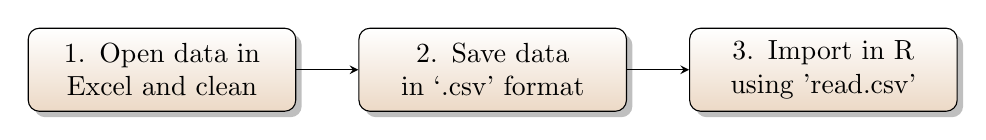
\begin{tikzpicture}[node distance=2.5cm, auto, >=stealth]
	\onslide<2->{
	\node[block] (a) {1. Open data in Excel and clean};}
	\onslide<3->{
	\node[block] (b)  [right of=a, node distance=4.2cm] {2. Save data in `.csv' format};
 	\draw[->] (a) -- (b);}
 	\onslide<4->{
 	\node[block] (c)  [right of=b, node distance=4.2cm]  {3. Import in R using 'read.csv'};
 	\draw[->] (b) -- (c);}
\end{tikzpicture}
\end{center}
\begin{columns}[t]
\onslide<2->{
\begin{column}{0.33\textwidth}
\begin{itemize}
\item Column names should be simple
\item Ensure all data will be easy to read
\end{itemize}
\end{column}}
\onslide<3->{
\begin{column}{0.33\textwidth}
\begin{itemize}
\item File, Save as .csv
\item Creates a comma separated file that looks like a spreadsheet
\item One spreadsheet at a time
\end{itemize}
\end{column}}
\onslide<4->{
\begin{column}{0.33\textwidth}
\begin{itemize}
\item header = T
\item See ?read.csv for list of function options
\item Remember to assign a name
\end{itemize}
\end{column}}
\end{columns}
\end{frame}

%%%%%%
\begin{frame}{Data organization}
Excel files can also be imported directly into R without converting to a .csv file \\~\\
However, this is not as intuitive as one would expect since .xls files are a proprietary format \\~\\
There are several packages for importing excel files: Here's a nice \href{http://www.r-bloggers.com/a-million-ways-to-connect-r-and-excel/}{summary} \\~\\
Try using the \href{http://cran.r-project.org/web/packages/gdata/gdata.pdf}{gdata} package on your own, this also requires an installation of \href{http://strawberryperl.com/}{Strawberry Perl}\\~\\
Our workshop will not use methods that require direct import of Excel files - we will always use a .csv or .txt format for simplicity
\end{frame}

%%%%%%
\begin{frame}[fragile,shrink]{Data organization}
If the data you want to import are a text file... open it, how are the columns separated?
\begin{itemize}
\item comma... \verb!sep = ','!
\item tabs... \verb!sep = '\t'!
\item space... \verb!sep = ''!
\item arbitrary character\\~\\
\end{itemize}
\pause
Use the read.table function and identify the column delimiter :
\begin{knitrout}\scriptsize
\definecolor{shadecolor}{rgb}{0.969, 0.969, 0.969}\color{fgcolor}\begin{kframe}
\begin{alltt}
\hlcom{# data not loaded, only 'a' from before}
\hlkwd{ls}\hlstd{()}
\end{alltt}
\begin{verbatim}
## [1] "a"
\end{verbatim}
\begin{alltt}
\hlcom{# load data as comma separated, assign to dat}
\hlcom{# make sure you are in the correct working directory}
\hlcom{# e.g., setwd('C:/my_directory') }
\hlstd{dat} \hlkwb{<-} \hlkwd{read.table}\hlstd{(}\hlstr{'dat_example.txt'}\hlstd{,}\hlkwc{sep} \hlstd{=} \hlstr{','}\hlstd{,} \hlkwc{header} \hlstd{= T)}
\hlkwd{ls}\hlstd{()}
\end{alltt}
\begin{verbatim}
## [1] "a"   "dat"
\end{verbatim}
\end{kframe}
\end{knitrout}
\end{frame}

%%%%%%
\begin{frame}[fragile,shrink]{Data exploration}
Now that the data are in our workspace, let's explore!\\~\\
View the first six rows
\begin{knitrout}\scriptsize
\definecolor{shadecolor}{rgb}{0.969, 0.969, 0.969}\color{fgcolor}\begin{kframe}
\begin{alltt}
\hlkwd{head}\hlstd{(dat)}
\end{alltt}
\begin{verbatim}
##         datetimestamp do_mgl depth
## 1 2011-01-01 00:00:00     NA  1.54
## 2 2011-01-01 00:15:00     NA  1.53
## 3 2011-01-01 00:30:00     NA  1.52
## 4 2011-01-01 00:45:00     NA  1.51
## 5 2011-01-01 01:00:00     NA  1.50
## 6 2011-01-01 01:15:00     NA  1.48
\end{verbatim}
\end{kframe}
\end{knitrout}
View the last six rows
\begin{knitrout}\scriptsize
\definecolor{shadecolor}{rgb}{0.969, 0.969, 0.969}\color{fgcolor}\begin{kframe}
\begin{alltt}
\hlkwd{tail}\hlstd{(dat)}
\end{alltt}
\begin{verbatim}
##            datetimestamp do_mgl depth
## 2971 2011-01-31 22:30:00    9.6  1.49
## 2972 2011-01-31 22:45:00    9.8  1.50
## 2973 2011-01-31 23:00:00   10.7  1.50
## 2974 2011-01-31 23:15:00   10.8  1.51
## 2975 2011-01-31 23:30:00   10.8  1.52
## 2976 2011-01-31 23:45:00   10.8  1.52
\end{verbatim}
\end{kframe}
\end{knitrout}
\end{frame}
 
%%%%%%
\begin{frame}[fragile]{Data exploration}
What object class is the data?
\begin{knitrout}\scriptsize
\definecolor{shadecolor}{rgb}{0.969, 0.969, 0.969}\color{fgcolor}\begin{kframe}
\begin{alltt}
\hlkwd{class}\hlstd{(dat)}
\end{alltt}
\begin{verbatim}
## [1] "data.frame"
\end{verbatim}
\end{kframe}
\end{knitrout}
What are the dimensions of the data frame?
\begin{knitrout}\scriptsize
\definecolor{shadecolor}{rgb}{0.969, 0.969, 0.969}\color{fgcolor}\begin{kframe}
\begin{alltt}
\hlkwd{dim}\hlstd{(dat)}
\end{alltt}
\begin{verbatim}
## [1] 2976    3
\end{verbatim}
\begin{alltt}
\hlkwd{nrow}\hlstd{(dat)}
\end{alltt}
\begin{verbatim}
## [1] 2976
\end{verbatim}
\begin{alltt}
\hlkwd{ncol}\hlstd{(dat)}
\end{alltt}
\begin{verbatim}
## [1] 3
\end{verbatim}
\end{kframe}
\end{knitrout}
The data contain 2976 rows and 3 columns, is this correct?
\end{frame}

%%%%%%
\begin{frame}[fragile]{Data exploration}
Can we get a summary of the data frame?
\pause
\begin{knitrout}\scriptsize
\definecolor{shadecolor}{rgb}{0.969, 0.969, 0.969}\color{fgcolor}\begin{kframe}
\begin{alltt}
\hlkwd{summary}\hlstd{(dat)}
\end{alltt}
\begin{verbatim}
##              datetimestamp      do_mgl         depth     
##  2011-01-01 00:00:00:   1   Min.   : 7.5   Min.   :0.70  
##  2011-01-01 00:15:00:   1   1st Qu.: 9.5   1st Qu.:1.02  
##  2011-01-01 00:30:00:   1   Median :10.2   Median :1.21  
##  2011-01-01 00:45:00:   1   Mean   :10.1   Mean   :1.19  
##  2011-01-01 01:00:00:   1   3rd Qu.:10.7   3rd Qu.:1.36  
##  2011-01-01 01:15:00:   1   Max.   :12.5   Max.   :1.69  
##  (Other)            :2970   NA's   :431    NA's   :2
\end{verbatim}
\end{kframe}
\end{knitrout}
Summary returns different information depending on the class of each column\\~\\
The first column is considered a `factor' and simple counts are returned\\~\\
The other two columns are `numeric' and five number summaries are returned, including the number of observations with NA (or missing) values
\end{frame}

%%%%%%
\begin{frame}[fragile]{Data exploration}
Individual summmaries of variables are also possible\\~\\
How do we obtain variables of interest?
\small
\begin{knitrout}\scriptsize
\definecolor{shadecolor}{rgb}{0.969, 0.969, 0.969}\color{fgcolor}\begin{kframe}
\begin{alltt}
\hlkwd{names}\hlstd{(dat)}
\end{alltt}
\begin{verbatim}
## [1] "datetimestamp" "do_mgl"        "depth"
\end{verbatim}
\end{kframe}
\end{knitrout}
\normalsize
We can get a variable directly using \$ or via indexing with [,]
\small
\begin{knitrout}\scriptsize
\definecolor{shadecolor}{rgb}{0.969, 0.969, 0.969}\color{fgcolor}\begin{kframe}
\begin{alltt}
\hlcom{# these all do the same thing}

\hlcom{# get using $}
\hlstd{dat}\hlopt{$}\hlstd{do_mgl}

\hlcom{# get using [row, column] with variable name}
\hlstd{dat[,} \hlstr{'do_mgl'}\hlstd{]}

\hlcom{# get using [row, column] with column index}
\hlstd{dat[,} \hlnum{2}\hlstd{]}
\end{alltt}
\end{kframe}
\end{knitrout}
\end{frame}

%%%%%%
\begin{frame}[fragile]{Data exploration}
Just as we had summaries of the data frame, we can get summaries of individual variables
\begin{knitrout}\scriptsize
\definecolor{shadecolor}{rgb}{0.969, 0.969, 0.969}\color{fgcolor}\begin{kframe}
\begin{alltt}
\hlkwd{summary}\hlstd{(dat}\hlopt{$}\hlstd{do_mgl)}
\end{alltt}
\begin{verbatim}
##    Min. 1st Qu.  Median    Mean 3rd Qu.    Max.    NA's 
##     7.5     9.5    10.2    10.1    10.7    12.5     431
\end{verbatim}
\end{kframe}
\end{knitrout}
Or specific information...
\begin{knitrout}\scriptsize
\definecolor{shadecolor}{rgb}{0.969, 0.969, 0.969}\color{fgcolor}\begin{kframe}
\begin{alltt}
\hlcom{# note use of na.rm = T, you must specify how to handle missing values}
\hlkwd{mean}\hlstd{(dat}\hlopt{$}\hlstd{do_mgl,} \hlkwc{na.rm} \hlstd{= T)}
\end{alltt}
\begin{verbatim}
## [1] 10.15
\end{verbatim}
\begin{alltt}
\hlkwd{range}\hlstd{(dat}\hlopt{$}\hlstd{do_mgl,} \hlkwc{na.rm} \hlstd{= T)}
\end{alltt}
\begin{verbatim}
## [1]  7.5 12.5
\end{verbatim}
\begin{alltt}
\hlkwd{var}\hlstd{(dat}\hlopt{$}\hlstd{do_mgl,} \hlkwc{na.rm} \hlstd{= T)}
\end{alltt}
\begin{verbatim}
## [1] 0.8342
\end{verbatim}
\end{kframe}
\end{knitrout}
\end{frame}

%%%%%%
\begin{frame}[fragile]{Data exploration}
Text-based summaries of our data are nice, but we should also visualize:
\begin{itemize}
\item How are our data distributed?
\item Are there any outliers or extreme observations?
\item How do our variables compare?\\~\\
\end{itemize}
R has many built in functions for data exploration and plotting
\begin{itemize}
\item hist - plots a histogram (binned densities of continuous values)
\item qqplot - comparison of a variable to a normal distribution
\item barplot - for bar plots...
\item plot - bivariate comparison of two variables
\item Much, much more...
\end{itemize}
\end{frame}

%%%%%%
\begin{frame}[fragile]{Data exploration}
Let's examine the distribution of dissolved oxygen measurements
\begin{columns}
\begin{column}{0.6\textwidth}
\begin{knitrout}\scriptsize
\definecolor{shadecolor}{rgb}{0.969, 0.969, 0.969}\color{fgcolor}\begin{kframe}
\begin{alltt}
\hlkwd{hist}\hlstd{(dat}\hlopt{$}\hlstd{do_mgl)}
\end{alltt}
\end{kframe}

{\centering 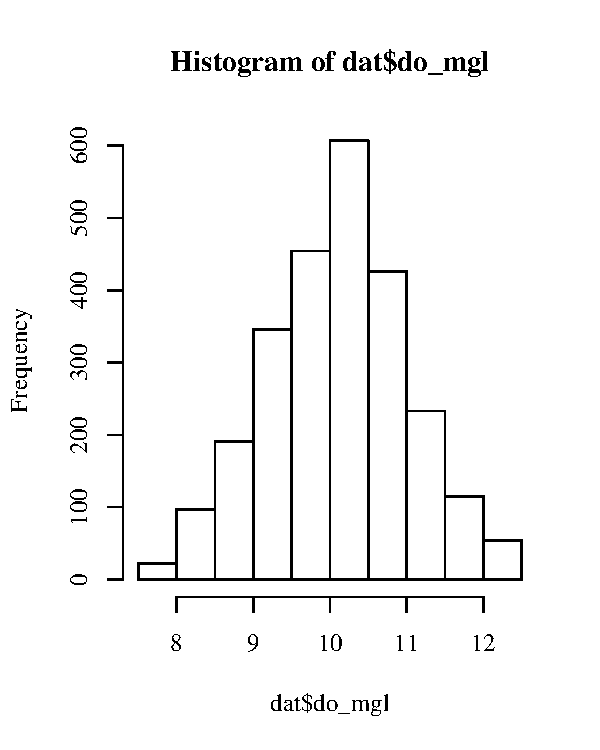
\includegraphics[width=0.7\textwidth]{figure/histdo} 

}



\end{knitrout}
\end{column}
\begin{column}{0.4\textwidth}
For example, $\approx$ 600 observations have DO values from, 10--10.5 mg L$^{-1}$
\end{column}
\end{columns}
\end{frame}

%%%%%%
\begin{frame}[fragile]{Data exploration}
Boxplots are also useful for looking at a distribution
\begin{columns}
\begin{column}{0.6\textwidth}
\begin{knitrout}\scriptsize
\definecolor{shadecolor}{rgb}{0.969, 0.969, 0.969}\color{fgcolor}\begin{kframe}
\begin{alltt}
\hlkwd{boxplot}\hlstd{(dat}\hlopt{$}\hlstd{do_mgl)}
\end{alltt}
\end{kframe}

{\centering 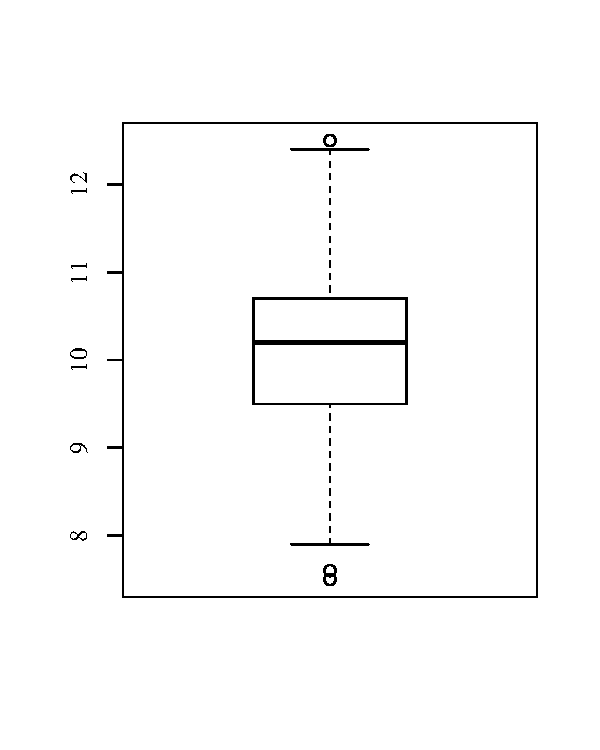
\includegraphics[width=0.7\textwidth]{figure/histbox} 

}



\end{knitrout}
\end{column}
\begin{column}{0.4\textwidth}
Let's make it look better...
\end{column}
\end{columns}
\end{frame}

%%%%%%
\begin{frame}[fragile]{Data exploration}
Boxplots are also useful for looking at a distribution
\begin{knitrout}\scriptsize
\definecolor{shadecolor}{rgb}{0.969, 0.969, 0.969}\color{fgcolor}\begin{kframe}
\begin{alltt}
\hlcom{# a nicer looking boxplot}
\hlkwd{boxplot}\hlstd{(dat}\hlopt{$}\hlstd{do_mgl,}
  \hlkwc{ylab} \hlstd{=} \hlstr{'DO (mg/L)'}\hlstd{,}
  \hlkwc{main} \hlstd{=} \hlstr{'Boxplot of dissolved oxygen'}\hlstd{,}
  \hlkwc{col} \hlstd{=} \hlstr{'lightblue'}
  \hlstd{)}
\hlcom{# see ?boxplot for all options}
\end{alltt}
\end{kframe}

{\centering 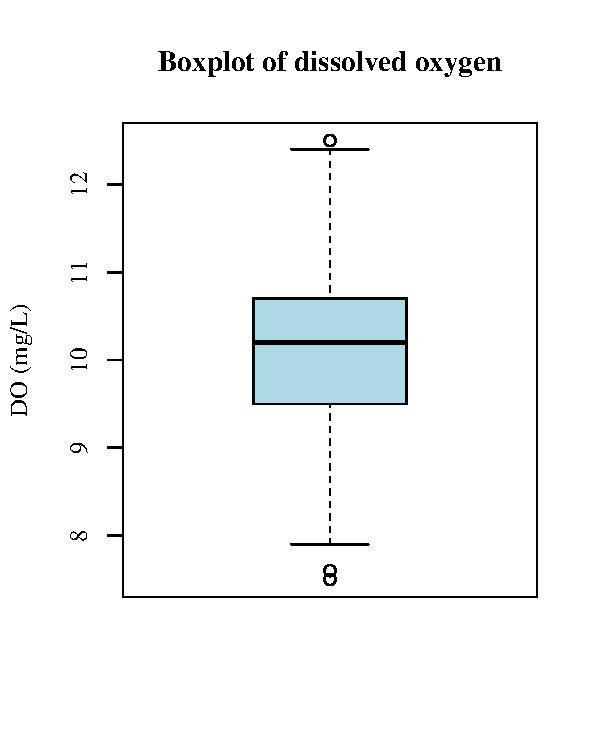
\includegraphics[width=0.35\textwidth]{figure/histbox2} 

}



\end{knitrout}
\end{frame}

%%%%%%
\begin{frame}[fragile]{Data exploration}
Values beyond the whiskers in a boxplot are considered outliers\\~\\
We can use the boxplot function to identify outliers...
\begin{knitrout}\scriptsize
\definecolor{shadecolor}{rgb}{0.969, 0.969, 0.969}\color{fgcolor}\begin{kframe}
\begin{alltt}
\hlcom{# find the outliers using boxplot}
\hlstd{myplot} \hlkwb{<-} \hlkwd{boxplot}\hlstd{(dat}\hlopt{$}\hlstd{do_mgl,} \hlkwc{plot} \hlstd{= F)}
\hlstd{myplot}\hlopt{$}\hlstd{out}
\end{alltt}
\begin{verbatim}
## [1]  7.6  7.6  7.5  7.6 12.5 12.5 12.5
\end{verbatim}
\end{kframe}
\end{knitrout}
This gives us the actual value, now we need to find them in our data \\~\\
\begin{knitrout}\scriptsize
\definecolor{shadecolor}{rgb}{0.969, 0.969, 0.969}\color{fgcolor}\begin{kframe}
\begin{alltt}
\hlcom{# find the rows of the outliers}
\hlstd{outlier} \hlkwb{<-} \hlstd{myplot}\hlopt{$}\hlstd{out}
\hlstd{out_row} \hlkwb{<-} \hlkwd{which}\hlstd{(dat}\hlopt{$}\hlstd{do_mgl} \hlopt \hlstd{outlier)}
\hlstd{out_row} \hlcom{#these are the row number of the outliers}
\end{alltt}
\begin{verbatim}
## [1]  704 1001 1002 1003 1322 1440 1441
\end{verbatim}
\end{kframe}
\end{knitrout}
\end{frame}
 
%%%%%%
\begin{frame}[fragile,shrink]{Data exploration}
You can treat outliers as you wish
\begin{knitrout}\scriptsize
\definecolor{shadecolor}{rgb}{0.969, 0.969, 0.969}\color{fgcolor}\begin{kframe}
\begin{alltt}
\hlstd{dat[out_row, ]} \hlcom{# view the outliers}
\end{alltt}
\begin{verbatim}
##            datetimestamp do_mgl depth
## 704  2011-01-08 07:45:00    7.6  1.20
## 1001 2011-01-11 10:00:00    7.6  1.32
## 1002 2011-01-11 10:15:00    7.5  1.31
## 1003 2011-01-11 10:30:00    7.6  1.30
## 1322 2011-01-14 18:15:00   12.5  1.28
## 1440 2011-01-15 23:45:00   12.5  1.38
## 1441 2011-01-16 00:00:00   12.5  1.37
\end{verbatim}
\end{kframe}
\end{knitrout}
Remove them...
\begin{knitrout}\scriptsize
\definecolor{shadecolor}{rgb}{0.969, 0.969, 0.969}\color{fgcolor}\begin{kframe}
\begin{alltt}
\hlstd{dat[out_row,} \hlstr{'do_mgl'}\hlstd{]} \hlkwb{<-} \hlnum{NA}
\end{alltt}
\end{kframe}
\end{knitrout}
Replace with mean...
\begin{knitrout}\scriptsize
\definecolor{shadecolor}{rgb}{0.969, 0.969, 0.969}\color{fgcolor}\begin{kframe}
\begin{alltt}
\hlstd{dat[out_row,} \hlstr{'do_mgl'}\hlstd{]} \hlkwb{<-} \hlkwd{mean}\hlstd{(dat}\hlopt{$}\hlstd{do_mgl,} \hlkwc{na.rm} \hlstd{= T)}
\end{alltt}
\end{kframe}
\end{knitrout}
Or do nothing...
\end{frame}

%%%%%%
\begin{frame}[fragile,shrink]{Data exploration}
The time series can be plotted to evaluate trends
\begin{knitrout}\scriptsize
\definecolor{shadecolor}{rgb}{0.969, 0.969, 0.969}\color{fgcolor}\begin{kframe}
\begin{alltt}
\hlcom{#first we have to convert the datetimestamp column}
\hlstd{dat}\hlopt{$}\hlstd{datetimestamp} \hlkwb{<-} \hlkwd{as.POSIXct}\hlstd{(dat}\hlopt{$}\hlstd{datetimestamp)}

\hlcom{# plot the time series, y vs x syntax}
\hlkwd{plot}\hlstd{(do_mgl} \hlopt{~} \hlstd{datetimestamp,} \hlkwc{data} \hlstd{= dat,} \hlkwc{type} \hlstd{=} \hlstr{'l'}\hlstd{)}
\end{alltt}
\end{kframe}

{\centering 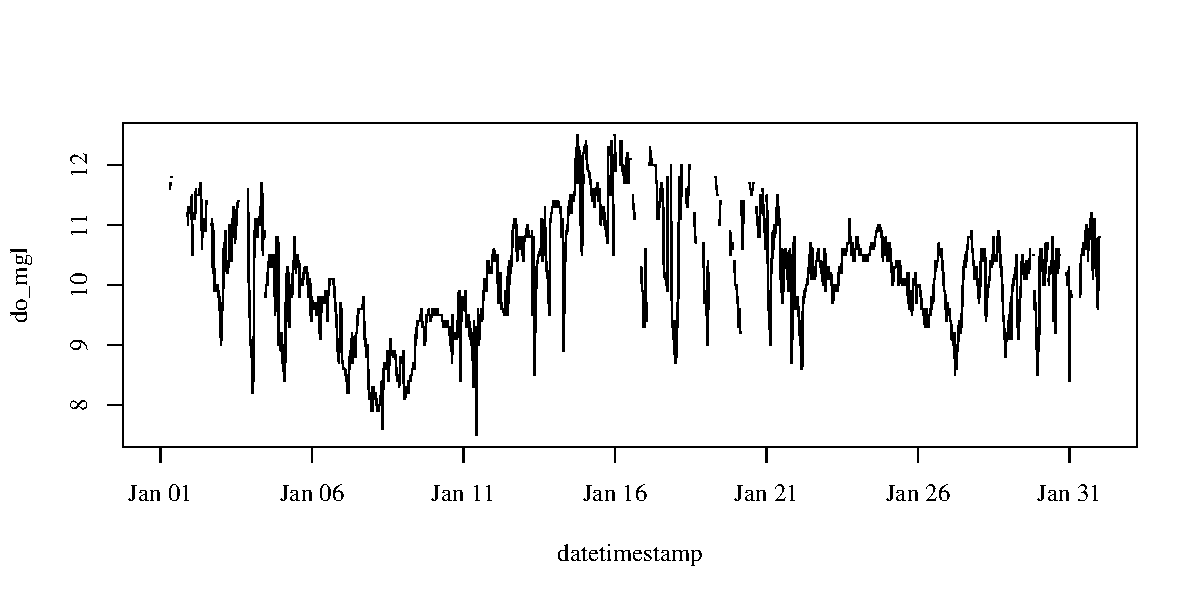
\includegraphics[width=\maxwidth]{figure/doseries} 

}



\end{knitrout}
\end{frame}

%%%%%%
\begin{frame}[fragile,shrink]{Data exploration}
We can also add our outliers to the plot
\begin{knitrout}\scriptsize
\definecolor{shadecolor}{rgb}{0.969, 0.969, 0.969}\color{fgcolor}\begin{kframe}
\begin{alltt}
\hlcom{# plot the time series}
\hlkwd{plot}\hlstd{(do_mgl} \hlopt{~} \hlstd{datetimestamp,} \hlkwc{data} \hlstd{= dat,} \hlkwc{type} \hlstd{=} \hlstr{'l'}\hlstd{)}

\hlcom{# use the out_row object from earlier to subset}
\hlstd{x} \hlkwb{<-} \hlstd{dat[out_row,} \hlstr{'datetimestamp'}\hlstd{]}
\hlstd{y} \hlkwb{<-} \hlstd{dat[out_row,} \hlstr{'do_mgl'}\hlstd{]}
\hlkwd{points}\hlstd{(x, y,} \hlkwc{col} \hlstd{=} \hlstr{'red'}\hlstd{)}
\end{alltt}
\end{kframe}

{\centering 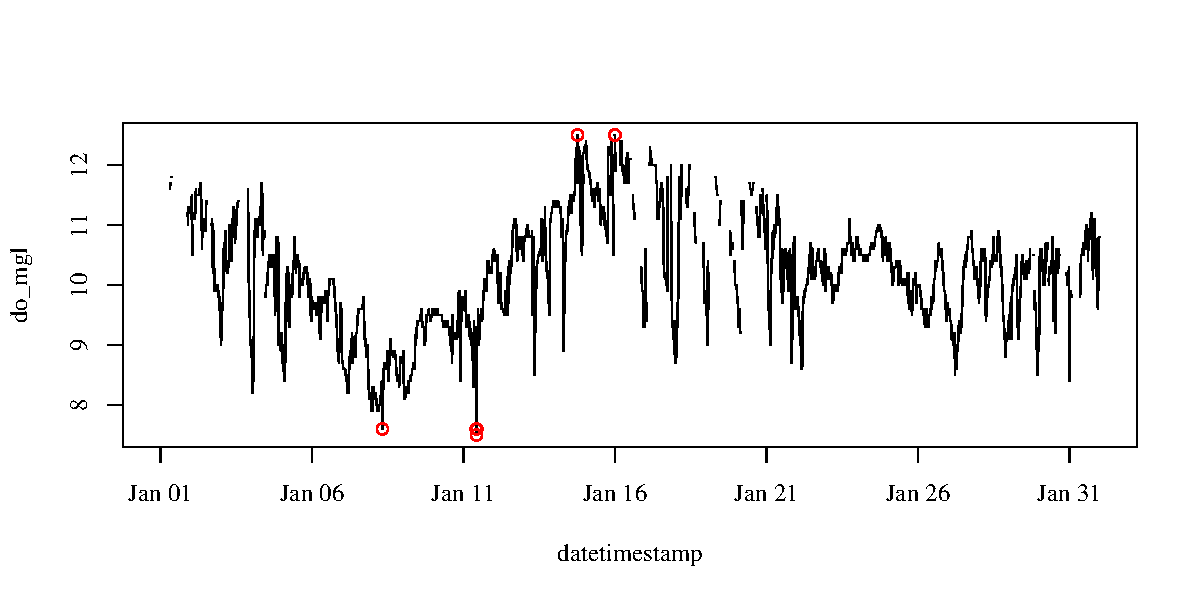
\includegraphics[width=\maxwidth]{figure/doseries2} 

}



\end{knitrout}
\end{frame}

%%%%%
\begin{frame}[fragile,shrink]{Data exploration}
What effect do these outliers have on the mean DO value for the time series?
\begin{knitrout}\scriptsize
\definecolor{shadecolor}{rgb}{0.969, 0.969, 0.969}\color{fgcolor}\begin{kframe}
\begin{alltt}
\hlcom{# the original dataset}
\hlstd{dat_orig} \hlkwb{<-} \hlstd{dat}\hlopt{$}\hlstd{do_mgl}

\hlcom{# dataset with outliers removed}
\hlstd{dat_remove} \hlkwb{<-} \hlstd{dat}\hlopt{$}\hlstd{do_mgl}
\hlstd{dat_remove[out_row]} \hlkwb{<-} \hlnum{NA}

\hlcom{# a boxplot comparison of the two datasets}
\hlkwd{boxplot}\hlstd{(dat_orig, dat_remove)}
\end{alltt}
\end{kframe}

{\centering 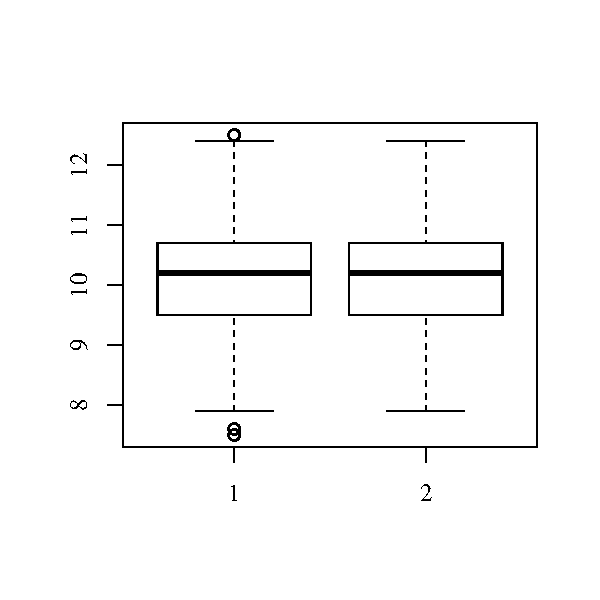
\includegraphics[width=0.35\textwidth]{figure/datcomp} 

}



\end{knitrout}
\end{frame}

%%%%%
\begin{frame}[fragile,shrink]{Data exploration}
We can test these differences more formally using a standard statistical test
\begin{knitrout}\scriptsize
\definecolor{shadecolor}{rgb}{0.969, 0.969, 0.969}\color{fgcolor}\begin{kframe}
\begin{alltt}
\hlcom{# a t-test, evaluates the null that the difference in means is zero}
\hlkwd{t.test}\hlstd{(dat_orig, dat_remove)}
\end{alltt}
\begin{verbatim}
## 
## 	Welch Two Sample t-test
## 
## data:  dat_orig and dat_remove
## t = -0.05, df = 5081, p-value = 0.9602
## alternative hypothesis: true difference in means is not equal to 0
## 95 percent confidence interval:
##  -0.05128  0.04873
## sample estimates:
## mean of x mean of y 
##     10.15     10.15
\end{verbatim}
\end{kframe}
\end{knitrout}
There is a 96.02\% probability that the difference in means between the datasets is equal to zero, due to random chance\\~\\
We should leave the outliers in the dataset...
\end{frame}

%%%%%%
\begin{frame}{Conclusions}
The previous examples are simple approaches to exploratory data analysis with R\\~\\
These were designed to get you comfortable using the R command-line\\~\\
The workshop will provide a comprehensive guide to exploring and working with time series data from SWMP\\~\\
Please see the additional resources slide in `intro\_to\_r.pdf' for more training information\\~\\
Questions: contact Marcus Beck (\href{mailto:beck.marcus@epa.gov}{beck.marcus@epa.gov}) or Todd O'Brien (\href{mailto:todd.obrien@noaa.gov}{todd.obrien@noaa.gov})
\end{frame}

\end{document}
